\chapter{Literature Review}
\label{chap:lit}
% \section{Hand Tracking Systems}
% Latent regression forest: structured estimation of 3d hand poses

% \section{Datasets}

This section will outline the state-of-the-art in hand tracking. Given the nature of this project, a particular focus is put on works that produce datasets for hand tracking, as well as systems that use depth sensors. As well as this, other works investigated include the related problem of full body pose estimation, as well as hand tracking with RGB sensors. The aim in this section is to establish the general idea of what a modern hand tracking system entails, how these systems adapt to the real world, and any relevant gaps and problems in research.

\section{Previous Work}
\subsection{Data}
% \subsubsection{Hand datasets}
A common issue highlighted in literature is a lack of data \cite{armagan2020measuring}, leading many to produce new datasets for training hand tracking systems. There are broadly two kinds of hand tracking datasets. Firstly, depth-based datasets consist of depth images. Such images capture the depth information of the scene. Secondly, RGB-based datasets consist of colour images of the hand. Some systems use both depth and RGB images for hand tracking. Different datasets also employ different labelling regimens. Most datasets aim to annotate the 3D locations of keypoints. These keypoints consist of certain points of interest in the hand, typically the knuckles, wrist, and finger joints. Some datasets only annotate the 2D keypoint locations which is easier to produce, while most datasets discussed here annotate the 3D keypoint locations, as this provides a richer feature space to extract information about the hand, although it is more difficult to estimate 3D keypoints as opposed to 2D keypoints. Another labelling strategy is to segment the images into different parts, such as the region that contains particular fingers. The other distinction between hand tracking datasets is whether they are real or synthetic datasets.

The {\slshape NYU} dataset \cite{tompson2014real}, which is based on depth images is one of the first modern hand-tracking datasets. The authors describe a comprehensive pipeline for acquiring data, and then training a {\slshape convolutional neural network} (CNN) with that data, to produce a system that can infer the continuous pose shape of a hand. In the dataset creation pipeline, the hand is first segmented using a {\slshape randomised decision forest}. Then using an initial approximation of the pose parameters, a {\slshape particle swarm optimisation} algorithm is used whereby a candidate pose is used to generate a synthetic image using an {\slshape linear blend skinning} (LBS) model. The captured image is compared against the generated image using an objective function and the candidate pose is updated using a loss function. The {\slshape Nelder–Mead} method is used to refine the pose estimates. The initial guess of the first frame is manually annotated, and is passed in a chain to each subsequent frame to be labelled. Their dataset is from two subjects, with 72,000 training, and 8,000 test images.

Two new datasets are introduced in \cite{sharp2015accurate}. Their first dataset, {\slshape FingerPaint} consists depth of images of hands whose groundtruth consist of pixel-wise classifications of the fingers of the hand as well as the palm, describing what region of the hand it belongs to, such as the palm, index finger, etc. The ground truth does not describe the location of keypoints. The annotations are generated with the help of an RGB sensor also recording the hand sequence. The hands are `painted' and segmented with a colour segmentation algorithm to generate the labels, with any errors corrected manually. This dataset is not intended for training, instead just for evaluating the performance of a hand tracking system. The other dataset that they generate is called {\slshape Synthetic}, which consists of 1000 synthetic depth images rendered using a 3D mesh model. Unlike {\slshape FingerPaint}, these images are not in a sequence and are in random articulations. Exact details are not available, but it is likely that the groundtruth consists of 3D keypoint positions.

% To be expanded!
Expanding on the labelling strategy of \cite{tompson2014real}, \cite{sun2015cascaded} introduce the {\slshape MSRA} dataset of 76,500 depth images from 9 subjects for evaluating a hand tracking system. Each of the subjects recorded were asked to produce 17 different poses which the authors say are mostly drawn from American Sign Language. The ground truth is generated from another hand tracking system and manually corrected for any errors.

\cite{tang2016latent} introduce a dataset consisting of 180,000 depth images with 3D keypoint annotation. In what they call the {\slshape ICVL} dataset, it contains hand poses from 10 different subjects. Each of the subjects are presented with the same 26 poses to recreate with their hands. They use Intel’s {\slshape Creative Interactive Gesture Camera} to capture the data which they say provides far better depth image quality than previous technologies. The annotation is generated by fitting a point cloud (a series of 3D points which together describe the shape of a 3D surface) version of the depth image to an articulated synthetic hand model. The authors highlight that this annotation system often fails at difficult poses, which means that their dataset largely contains easy frontal poses (where the camera is positioned in front of the subject). To account for this limitation, they compare their dataset with the {\slshape Synthetic} dataset introduced by \cite{sharp2015accurate}.

{\slshape BigHand2.2M} \cite{yuan2017bighand2} is the first large scale hand tracking dataset, containing ~2.2 million annotated depth images of hands for training and evaluating a hand tracking model. They use Intel's {\slshape RealSense SR300}.Sample images can be seen in Figure \ref{figs:lr:bighand}. They highlight the lack of available datasets for hand tracking, and hypothesise the reason is the lack of scalable methods for annotation. They claim existing automatic methods are not accurate enough, or that they compromise the dataset (such as the use of gloves to aid annotation). They say that manual annotation is too slow to make a dataset sufficiently large. They introduce a new capture method for annotation where the hand is fitted with magnets on each fingertip as well as the palm. With a depth camera capturing the data, the annotations are generated using magnetic sensors. They produce 21 3D keypoints using {\slshape inverse kinematics} of the hand to generate the subsequent annotations. Their dataset is from ten subjects.

\begin{figure}
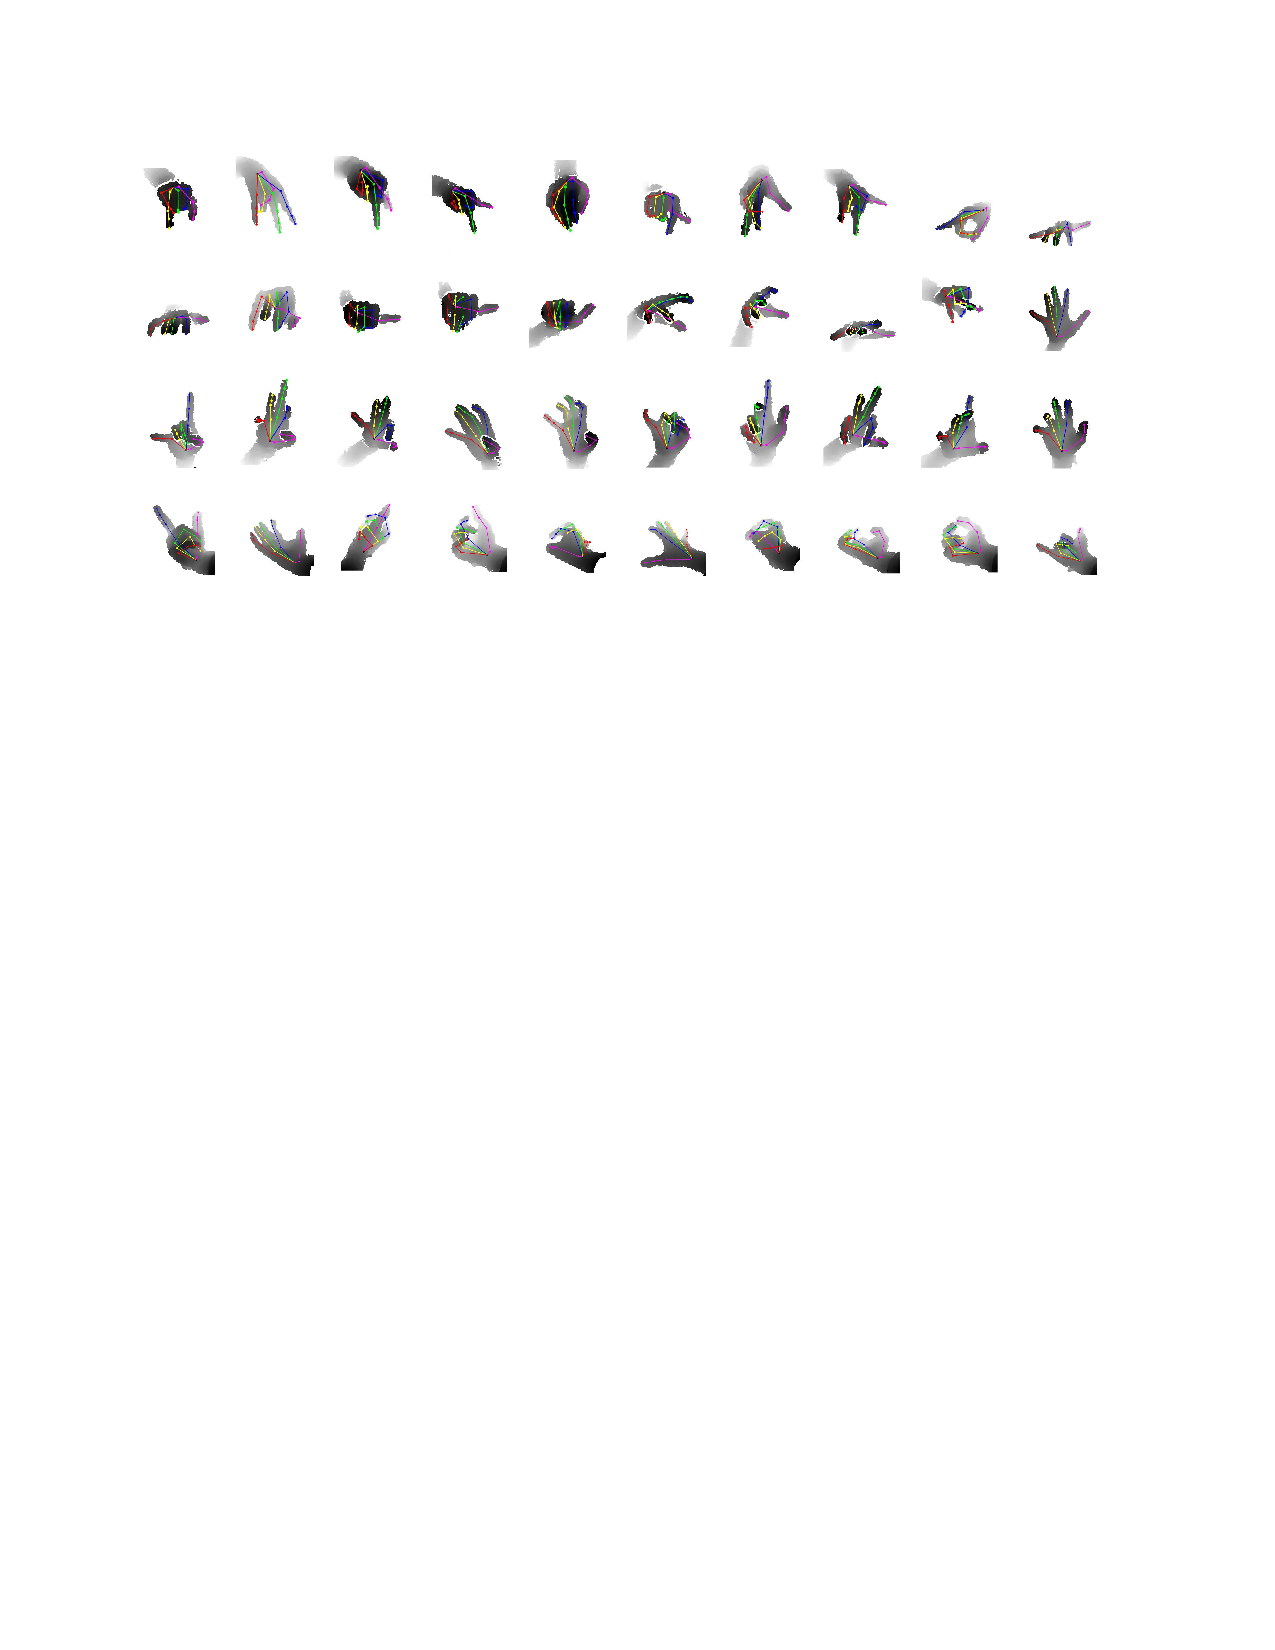
\includegraphics[width=\linewidth]{figs/general/bighand22m.pdf}
\caption{Sample images from the BigHand2.2M dataset with the annotation superimposed. Image taken from the original paper \cite{yuan2017bighand2}.}
\label{figs:lr:bighand}
\end{figure}

\cite{mueller2017real} introduce a new RGB and depth synthetic dataset, {\slshape SynthHands}. They define an egocentric viewpoint as the camera perspective of the hands as is seen from the head or chest. The reasoning behind making such a dataset is that it is challenging to capture the real world annotations of hands, and that existing datasets lack hand-object interactions and realistic hand poses, nor do they show real world noise and backgrounds. They highlight that annotating an egocentric dataset is particularly challenging due to the increased likelihood of self occlusion, which is where the hand blocks part of itself from the camera view. The gestures rendered in the synthetic dataset are generated from real gestures captured from a human hand, with the camera retargeted to an egocentric viewpoint. As well as this, the synthetic hands have artificial interactions with objects, and the background is composited with different scenarios including desktops, offices, corridors, and kitchens.

\cite{malik2018deephps} propose a new dataset, {\slshape SynHand5M}, which contains 5 million synthetically generated depth images of hands in different poses, and camera viewpoints. They claim this approach to be superior to \cite{yuan2017bighand2} and \cite{romero2017embodied}, since they are both based on the data of a small amount of subjects, the nature of their synthetic data generation algorithm means they can vary the shape of a hand, which cannot be done with real data. They also claim that since the data is synthetically generated, the groundtruth is perfect. Their goal in making this dataset is to cover most, if not all possible articulations, shapes, and camera perspectives. To this end, in order to ensure that the hand shapes are realistic, they use limits defined by an anthropometric database. They also set limits to the articulations of the hand. This is because it is easy to deform the synthetic hand into shapes that a real world hand would not be able to achieve, which could lead the hand tracking system that trains on this dataset to learn unrealistic hand articulations. They admit that their specific implementation is not fully realistic, but claim that this is sufficient as a pretraining step for the CNN that they use for their hand-tracking system.

\cite{wang2018mask} highlight the lack of data available for training RGB based systems. They show that existing RGB based datasets are synthetic, or captured in a lab setting. Unlike depth images, RGB images have to have a background to simulate real life use, and the background has to vary too or else the model may just learn that background and it will not be able to segment other types of backgrounds. Their new dataset is called {\slshape OneHand10K} which consists of 11703 RGB images with varying backgrounds, and annotated for 21 2D keypoints. The groundtruth is manually annoted by at least three different people marking, and keypoints that are not visible in the dataset are not annotated.

\subsection{Rendering Methods}
A new full-body statistical model is introduced in \cite{romero2017embodied} called MANO. Built on previous full-body statistical models, MANO is compatible with mainstream computer graphics systems and allows synthetic poses using a set of shape and articulation parameters to model different body shapes and poses seen in real life respectively. MANO places a special emphasis on hands, the authors highlight that recent advances in full-body models have often neglected hands, given their complex articulated nature with respect to the rest of the human body. The model is learned by capturing the full body and hands separately. The hand model data is captured from 31 subjects performing 51 different actions including hand-object interaction. The combined model uses LBS, and the authors say that certain corrective blend shapes are used to mitigate the drawbacks of LBS. The model takes two parameters $\bm{\beta}$ and $\bm{\theta}$ which outputs 778 vertices describing the shape of a hand in 3D space. These vertices can then be put into a standard graphics pipeline for rendering. They use this mesh model to improve the hand rendering performance of the full body model SMPL \cite{loper2015smpl}.

\subsection{Hand Tracking Systems}
A hand tracking system is one that in general, takes a depth, RGB, or both images as an input and outputs a set of 2D or 3D coordinates showing the location of the hand's keypoints. Modern (within the last 3-4 years) systems typically employ some form of CNN architecture, however the basic architectures that have seen success in other tasks such as ordinary image classification are typically not enough and a more sophisticated model is required.

\subsubsection{2D CNN Approaches}
\cite{mueller2017real} approach the problem of hand pose estimation using a combination of RGB and depth cameras from an egocentric perspective as mentioned in the dataset discussion. They combine the RGB and depth images into a coloured depth image (RGBD) first, and from that crop the image to the {\slshape region of interest} (ROI, the part of the image that contains the hand, either a bounding box, or semantic segmention). This is done by passing the image into a CNN which outputs a heatmap. The centre of this heatmap is supposed to be the MCP joint of the middle finger (see Figure \ref{fig:sd:hand} for an illustration). In order to ensure that the location of the centre of the heatmap is temporally consistent, if the confidence of this centre is less than 0.1, and it is more than 30 pixels away from the centre of the previous image, they update the heatmap centre using the sum of the previous frame and the estimate of the current location based on the motion of previous frames that were marked as confident. In a special function, it locates the centre of this heatmap, and using the depth information, it removes pixels that are far away from a 3D Eucliadian perspective. From there, this cropped RGBD image, it is passed into a CNN to regreess the 3D keypoints, as well as a 2D heatmap of these keypoints. The regressed 3D keypoint coordinates are refined using a kinematic hand model, and further refined with the help of the 2D heatmap.

\cite{malik2018deephps} employs a two-stage CNN architecture where given a depth image, they aim to estimate the 3D keypoint locations of the hand, as well as a vertex mesh representing a reconstruction of the hand's surface. Within this CNN, there are three parallel steps for estimating: the hand articulation $\bm{\theta}$, hand shape $\bm{\beta}$ (these parameters are not to be confused with similar notation of MANO), and scale $\alpha$. Inside the same CNN, $\alpha$, $\bm{\beta}$, and $\bm{\theta}$ are then passed into a non-linear differentiable layer (which means that this layer can be trained with backpropagation together with the previous layers) that they call a {\slshape Hand Pose and Shape Layer}. This layer consists of stages to construct a hand representation using the shape parameters $\alpha$, $\bm{\beta}$, and they use the $\bm{\theta}$ then to reconstruct the hand pose using Linear Blend Skinning.

\cite{wang2018mask} approach the hand tracking problem in terms of discovering a set of 2D keypoints in an RGB image. They highlight the advances made in hand tracking using depth sensors and the comparative slowness in progress for RGB systems. Many existing systems rely on strict lighting and backgrounds. Their model is divided into two parts, both are fully-convolutional networks, where the first segments a silhouette (a pixel-wise segmentation of the image into foreground that contains the hand, and background that does not contain the hand), and the second regresses the 2D keypoints. They believe that this approach can be a step towards RGB-based systems for 3D keypoint estimation.

\cite{wan2019dual} address hand tracking in terms of estimating a large set of vertices that describe the surface of a human hand from a depth image. The authors argue that estimating a small set of keypoints is underconstrained, and that estimating the vertices of a hand has more useful applications. To this end, they propose a {\slshape fully convolutional network} (FCN) architecture that estimates these vertices. There are two consecutive hour-glass FCNs. The first FCN has two heads (outputs), one with a generic feature map, and one with estimates 2D mesh coordinates of the image. In a process the authors call {\slshape extension}, the feature map and 2D mesh estimation are combined and passed into another FCN to give an initial estimate of the 3D vertices. This initial estimate is refined using a kinematic model of the hand.

\cite{liu2019feature} introduce a novel feature boosting algorithm for a CNN network for inferring the 3D keypoints of an RGB image of a hand or human body. They introduce a new {\slshape long short-term dependence-aware} (LSTD) module that understands the relationship between different keypoints to boost the feature outputs of a CNN network. For example, the keypoint relationship between two different keypoints in the same finger are highly correlated, but less so with keypoints in other fingers of the same hand. They highlight that many existing pose estimation methods do not factor the relationship between keypoints, or use keypoint relationships to refine the estimate as a post processing stage. Their network can be stacked into multiple blocks to further refine the keypoint estimate. To account for the unreliability of the features generated by a CNN due to occlusions and textures in the RGB input image, they also introduce a {\slshape context consistency gate} to act as a gating mechanism to the LSTD module which analyses the input features in terms of their context with respect to their neighbouring keypoints, and adjusts any irregularities to improve the estimation of the keypoint locations overall. They claim that their results achieve state-of-the-art results on human body estimation datasets.

\subsubsection{3D CNN Approaches}

\cite{moon2018v2v, ge2018real} both propose similar systems where depth image representation of a hand, is inputted to a 3D CNN to predict the 3D keypoints of the hand. The depth image, a 2D pixel array is converted into a 3D voxel (a voxel is the 3D equivalent to 2D pixels) representation and then passed into the CNN for inference. The authors cite the fact that a depth image really conveys 3D information, and they hypothesise that passing in a 2D depth image into a 2D CNN discards the 3D data, leading to reduced performance. \cite{moon2018v2v} discuss this hypothesis by running four experiments; a depth image is used to infer 3D keypoints, a depth image is used to infer voxelised 3D keypoints, a voxelised depth image is used to infer 3D keypoints, and a voxelised depth image is used to infer voxelised 3D keypoints. Their experiments show that a voxelised depth image used to infer voxelised 3D keypoints delivers superior performance over the other methods, they call their new architecture {\slshape V2V-PoseNet}. \cite{ge2018real} investigates this hypothesis by running these four experiments. Firstly a depth image is passed into a CNN to estimate the heatmap for each keypoint location. Second, the voxel representation of the hand is used to generate multiple depth map images from different perspectives and passed into a 2D CNN to estimate a series of heatmaps for keypoints for each input. Third, the single depth image is passed into a CNN to directly estimate the 3D keypoints. Fourth, the voxelised image is passed into a 3D CNN to estimate the 3D keypoint locatioins. \cite{malik2020handvoxnet} takes {\slshape V2V-PoseNet} one step further by also trying to estimate hand shape in addition to pose using more 3D CNN architectures in what they call {\slshape HandVoxNet}.

\begin{figure}
    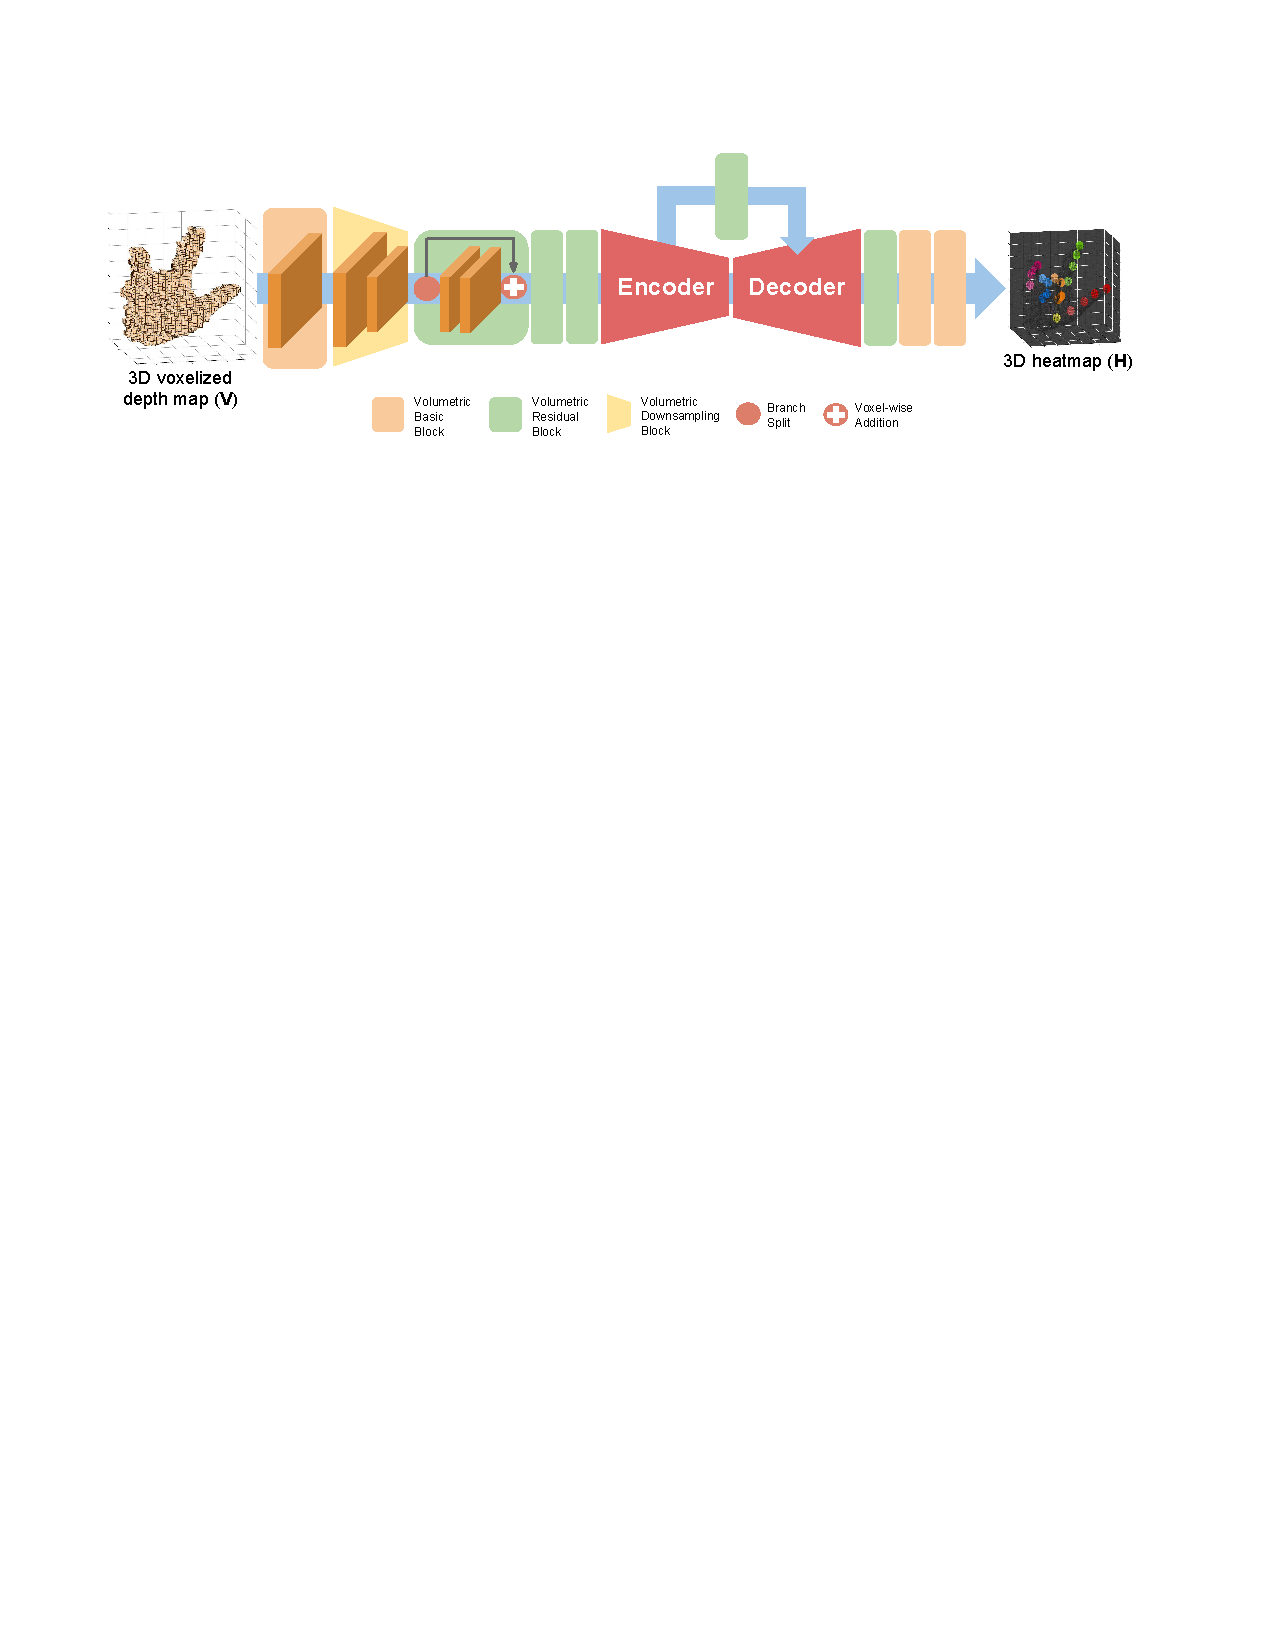
\includegraphics[width=\linewidth]{figs/general/v2v-posenet.pdf}
    \caption{An illustration of the V2V-Posenet model. Image taken from the original paper \cite{moon2018v2v}.}
    \label{fig:v2vposenet}
    \end{figure}

\subsubsection{Generative Approaches}
Generative Adversarial Networks (GANs) are a recent neural network architecture where two components are trained in tandem, a generator to generate synthetic data, and a discriminator to tell whether it is real or not \cite{karras2017progressive}. The idea is that both components engage in a race to outperform the other, and ultimately we get a good system for generating synthetic data, and a good system for telling whether that is real or fake by both networks working against each other.

\cite{he2019graphposegan} address hand tracking for RGB images by adopting this GAN approach. In this paper, the authors use the generator to estimate the hand pose in a two stage process where an initial estimate is generated, and further refined using a parametric hand model. The discriminator acts effectively as a loss function, distinguishing between the predicted keypoints and groundtruth.

\cite{oberweger2019generalized} highlight how many recent works in hand pose estimation rely on a 3D hand model as part of the estimation process. They hypothesise that this is not an ideal approach given that these hand models are simplified and do not take the actual anatomical characteristics of the hand into consideration. Given a depth image as an input, they aim to estimate a set of keypoints describing the hand articulation, which is achieved as follows. After obtaining a box-shaped ROI of the hand, this is passed into a CNN to give an initial estimate of the 3D coordinates, which is passed into another CNN model that generates a synthetic image, in a similar approach to the generator in \cite{he2019graphposegan}. The real and synthetic depth images are passed into another CNN that updates the estimate of the keypoints, which is passed back into the generator CNN again in an iterative process.

\cite{chen2020dggan} propose a simple GAN for RGB-based pose estimation. They highlight the recent advances made in hand pose estimation using depth images, but they believe RGB-based methods to be ultimately superior because RGB sensors are cheaper and more readily available. Combining these two ideas, they aim to train a system that generates a depth image from an input RGB image in one module. In the other module, the 2D keypoints are directly estimated on the RGB image, then the 3D keypoints are regressed from that. This estimate is then refined using the generated depth image. The generative component needs to be trained with paired RGB and depth images, but it can then be trained on RGB images alone after that and they claim that the generative component can improve the estimate versus using RGB alone such as \cite{wang2018mask}.

\subsubsection{Cascaded Regressors}
\cite{sun2015cascaded} highlight recent successes in full body classification algorithms that classify the body into different regions based on what body part that they belong to, but that this approach does not work well for hands. They believe that this is because full body images are easy to classify, they tend to be all frontal-based. Hand images in contrast tend to have more varied camera angles and the hand is capable of deforming in far more diverse orientations. They therefore believe that regressing the pose of the hand, that is estimating the locations of 3D keypoints describing the locations of certain parts of a hand in 3D space is a more principled approach to the problem. They believe however that current regression techniques such as CNNs do not have the capacity to learn all of the possible variations in human hand poses. To address this hypothesis, they believe a cascaded regression approach for hand tracking is superior. Cascaded regression works by using a pipeline of weak regressors. They extend previous work for 2D cascaded hand pose regressors into 3D.

\cite{tang2018opening} address the problem that modern hand tracking systems are typically `black box' systems. That is, that the hand is passed into some model and it outputs the parameters without us knowing what is actually going on inside the system beyond the basic mathematics. This is a general problem within machine learning. They specifically address this issue for {\slshape analysis by synthesis} depth hand tracking systems such as \cite{sharp2015accurate}. In a process that they call {\slshape hierarchical sampling optimisation}, it uses knowledge of the hands structure to estimate the keypoints of the hands in a hierarchal way from the wrist towards the fingertips. Then, like \cite{sharp2015accurate}, this is used to render a synthetic version of the hand and compared against the original depth image using a scoring function.

\cite{yoo2019capturing} propose a hierarchal CNN for estimating the keypoints of a hand from a depth image. They highlight the progress made in accurate hand tracking in terms of reduced error, but also highlight the fact that some of the more accurate systems have a high computational overhead, particularly V2V-Posenet \cite{moon2018v2v}. Their system passes a depth image through an encoder, then the keypoints for the thumb, palm, and each finger are separately estimated in discrete CNN blocks to output 3D keypoints. Their system is more accurate than all of the systems that they survey except for \cite{li2019point, moon2018v2v}, however it is still faster than them.

\subsubsection{Mesh Recovery}
\cite{sharp2015accurate} introduce an {\slshape analysis by synthesis} approach for hand tracking. {\slshape Analysis by synthesis} is an approach to computer vision that uses {\slshape Bayesian inference}. This idea posits traditional machine learning where a model learns from data as `bottom up' processing, and they argue that we can gain more accurate insights about a problem by also considering a `top down' approach \cite{yuille2006vision}. The idea is that given an input image, an attempt is made to reverse the process of how that image was generated. In a simple example of classifying a pattern of text, this method says that we should separate this problem into components such as the probability of the font, noise, overlap, obstruction etc to get towards the core problem, that is: what the actual text is. In terms of hand tracking, this approach works by taking a depth image as an input, first segmenting the ROI. Then, the global rotation and subsequently local articulation are estimated to generate a series of candidate poses which are rendered into synthetic images. This synthetic image can then be compared against the original using a simple pixel-wise MSE function to choose the best one. This initial estimate is then refined using {\slshape particle swarm optimisation} combined with information from previous frames in the same video sequence.

\cite{baek2019pushing} uses the MANO model \cite{romero2017embodied} at the centre of their hand tracking system. Their system aims to predict 778 3D vertices describing a hand shape from an RGB input, in a similar `top down' approach to hand tracking as \cite{sharp2015accurate}. Instead of trying to predict this directly, they have a three-stage pipeline employing CNN architecture to achieve this. The first stage consists of two parts; one CNN generates a 2048-dimensional feature vector of the foreground of the image containing the hand, and another CNN estimates the 21 2D keypoints of the hand. A second CNN takes these features and keypoints as an input and outputs a 63-dimensional vector. The first 45 parameters are the articulation parameters for the MANO model $\bm{\theta}$, the next 10 are the MANO shape parameters $\bm{\beta}$, the next four are the camera rotation in quaternion space, one for scale, and the final three are for the camera translation. As previously described, the MANO model outputs 778 vertices given the articulation and shape parameters. The 778 vertex output can then be rotated, scaled, and translated as appropriate using the rotation, scale, and translation parameters. These 778 vertices are then passed to a regressor to obtain 21 keypoints in 3D space.

\subsection{Related Tracking Systems}

\cite{hoffmann2019learning} looks at the problem of full-body tracking. The authors specifically address the problem of the lack of training data for full-body tracking for RGB-based systems. Using the full-body version of MANO - (SMPL+H) \cite{romero2017embodied}, they produce two datasets, one containing fully-synthetic data, and one that is combined with a real dataset as an effective augmentation strategy. A large emphasis in the paper is trying to generate photo-realistic data, given that this is an RGB-based system. The generation of photorealistic data is not a problem limited to synthetic and is a general problem in computer graphics. One of the important insights about synthetic data from the paper is that some synthetically-generated images can convey more information than others. They use Mask R-CNN for segmentation and an existing model to generate shape parameters. To aid in training with synthetic data, they propose an adversarial approach which they call a `student teacher framework'. In this framework, synthetic images are grouped into ten groups based on camera position and the distance of a person to the camera. In training, a real image that has the highest loss per keypoint in the previous $N$ images is used to determine which type of synthetic image to use for training to ensure the network trains on the most difficult synthetic images.

% , and that only more difficult to train samples to limit the use of synthetic data
% Potentially i

% RAW -->


\section{The Modern Hand Tracking System}
% \begin{figure}
% \centering
% \includegraphics[width=250px]{figs/general/churchill_vsign.jpg}
% \caption{Image obtained from the {\slshape UK War Office Second World War Official Collection}. This illustrates the V sign, and the ambiguity between a polite, and rude gesture that a computer might misclassify. Winston Churchill famously was unaware of the vulgar meaning of the hand gesture.}
% \label{fig:lr:churchill}
% \end{figure}
The goal of hand tracking system is to find and extract information about a hand from an image containing one. That information must be sufficiently accurate to distinguish it from some other meaning. 

% Human hands play an intimate part in human communication, and many cultures have different etiquettes for what certain hand gestures mean. For example, the hand {\slshape V sign} (see Figure \ref{fig:lr:churchill} for an illustration) can convey two very different meanings depending on the global orientation of the hand. The most obvious application of a hand tracking system is for Virtual Reality, and Augmented reality headsets, as highlighted in many of the papers above. It is my opinion however that many new technologies find uses in ways that are hard to predict.

The general idea of modern hand tracking systems is as follows. Given an image (RGB and/or depth) that contains a hand, the image is first segmented to a Region of Interest (ROI) which is either semantically segmented (pixel-wise), or segmented with a tight bounding box. From there, the ROI is passed into a model that employs a neural network and sometimes an additional system to take the shape of a hand into account. From there, the system outputs a series of 3D points that describe the locations of certain  keypoints in the hand. This selection of keypoints can then be used to extract what information the hand is conveying in a low-dimensional environment, examples of this include \cite{devineau2018deep, nguyen2019skeleton, wang2019spfemd}. Most research effort appears to go into the use of depth cameras because the input is often less ambiguous than RGB images, and it preserves spatial information about the hand. This has been encouraged by the increasing popularity and quality of depth sensors. RGB-based hand tracking at this time appears far more elusive, given the increased ambiguity in the image due to diverse backgrounds, different skin colour, lighting, among other ambiguities. To give an example of this difference, it is easy to segment a depth image of a hand in front of a wooden floor by discarding all distant pixel values, in contrast with an RGB image, the skin color might be similar to the wooden floor so the segmentation task is far more challenging.

One issue highlighted in literature is the lack of data, many of these same papers also produce a dataset of their own to address this. Part of the problem is that it is difficult to make such datasets, as well as this, many of these datasets rely on few participants, usually in the order of 10-20 participants at most. The core of many modern hand tracking systems use CNNs, which require large datasets to train on. Exactly how much a hand tracking system needs is unknown, but other CNN tasks require in the order of 100,000-1,000,000 images or more. The reason for the lack of hand tracking data is that labelling it is difficult. It is far too labourious for a human to label a hand dataset at scale, and indeed the accuracy may not be good. Notably in \cite{wang2018mask}, they manually annotate their dataset, but this is only for 2D keypoints, and they simply omit keypoints that are occluded from the image. Other computer vision applications have seen a lot of real-world success because of the existance of large datasets for their domains, notably image classification\footnote{\url{http://image-net.org} (accessed 29th April 2020)}. For image classification tasks, it is far easier to label, notably the {\slshape reCAPTCHA} project got internet users to label images by combining the task with spam detection\footnote{\url{https://www.ted.com/talks/luis_von_ahn_massive_scale_online_collaboration} (accessed 29th April 2020)}. This is not possible with hand tracking however, and no scalable system exists to label a large hand tracking dataset without the help of an automatic method.

To automatically label datasets is a chicken and egg problem. The problem is thus: hand tracking systems need more data, and the data needs to be more accurate, but there is not sufficient data. This data can be captured relatively easily, but to label it at scale is practically impossible, therefore a hand tracking system should be used to annotate the data, but no such system exists. To get around this, past datasets have attached gloves, or other sensors to the hand to find the keypoint locations, but this then compromises the resultant images because the glove or sensor can be seen in the image. More recent examples have used a kinematic model of a hand to refine the estimate of the hand such as in the NYU dataset \cite{tompson2014real}. Other labelling efforts have involves placing discrete magnetic sensors on the fingertips and using an inverse kinematic model to estimate the other points\cite{yuan2017bighand2}. One problem with both of these datasets is that they both have a small amount of participants (two and ten respectively). This problem can be solved relatively easily. A problem that is harder to address however is the quality of the annotation, which goes back to the chicken and egg problem highlighted above. We can only hope that the annotation strategies of \cite{tompson2014real, yuan2017bighand2} are accurate. It is doubtful that the authors manually scrutinised each and every image. This is a big problem, because for any machine learning task, the system will only perform as well as the training data given to it. One way around this is to use synthetic data. This idea is explored in \cite{malik2018deephps}, when they create their {\slshape SynHand5M} dataset with perfect groundtruth, but they used a different hand model which they themselves admitted had limited realism. They also designed a new hand tracking system at the same time,  which means that their dataset has not been validated independently. Progress has been made since then with the advent of the MANO model\cite{romero2017embodied}. They specifically set out to address the problem of a lack of realism with hand data, and to the best of my knowledge, no further attempt at creating a large depth dataset has been attempted since {\slshape SynHand5M}.

These same problems are discussed by \cite{armagan2020measuring}, and they posit MANO as a synthetic data generation strategy to address these problems with existing hand data. As discussed in Section \ref{sec:intro:mot}, the research question of this project is particularly influenced by the {\slshape Hands 2019} challenge. Given these problems, this dissertation explores the most recent synthetic hand data generation technique, the MANO model to see how it can address them.

% To get around the problem of a lack of data, some methods use a hand model in the hand tracking system to refine the initial estimate in an iterative approach by fitting an input depth image against a rendered depth image based on the output of the estimated keypoints \cite{sharp2015accurate}. Other methods try to generate hand data synthetically \cite{mueller2017real,malik2018deephps,hoffmann2019learning}.